\section{WS2: Preparing the flying environment}

For flight testing of the crazyflies this project is using the Smart City environment which is part of the WCN Lab at Aalborg University. Smart City is a miniature city block consisting of traffic lanes and buildings and it uses Optitrack motion system for determining the position of the objects within its boundaries. As seen in Figure \ref{figure:smart_city_layout} the right-handed XYZ positioning system is used:

\begin{figure}[H]
\centering
 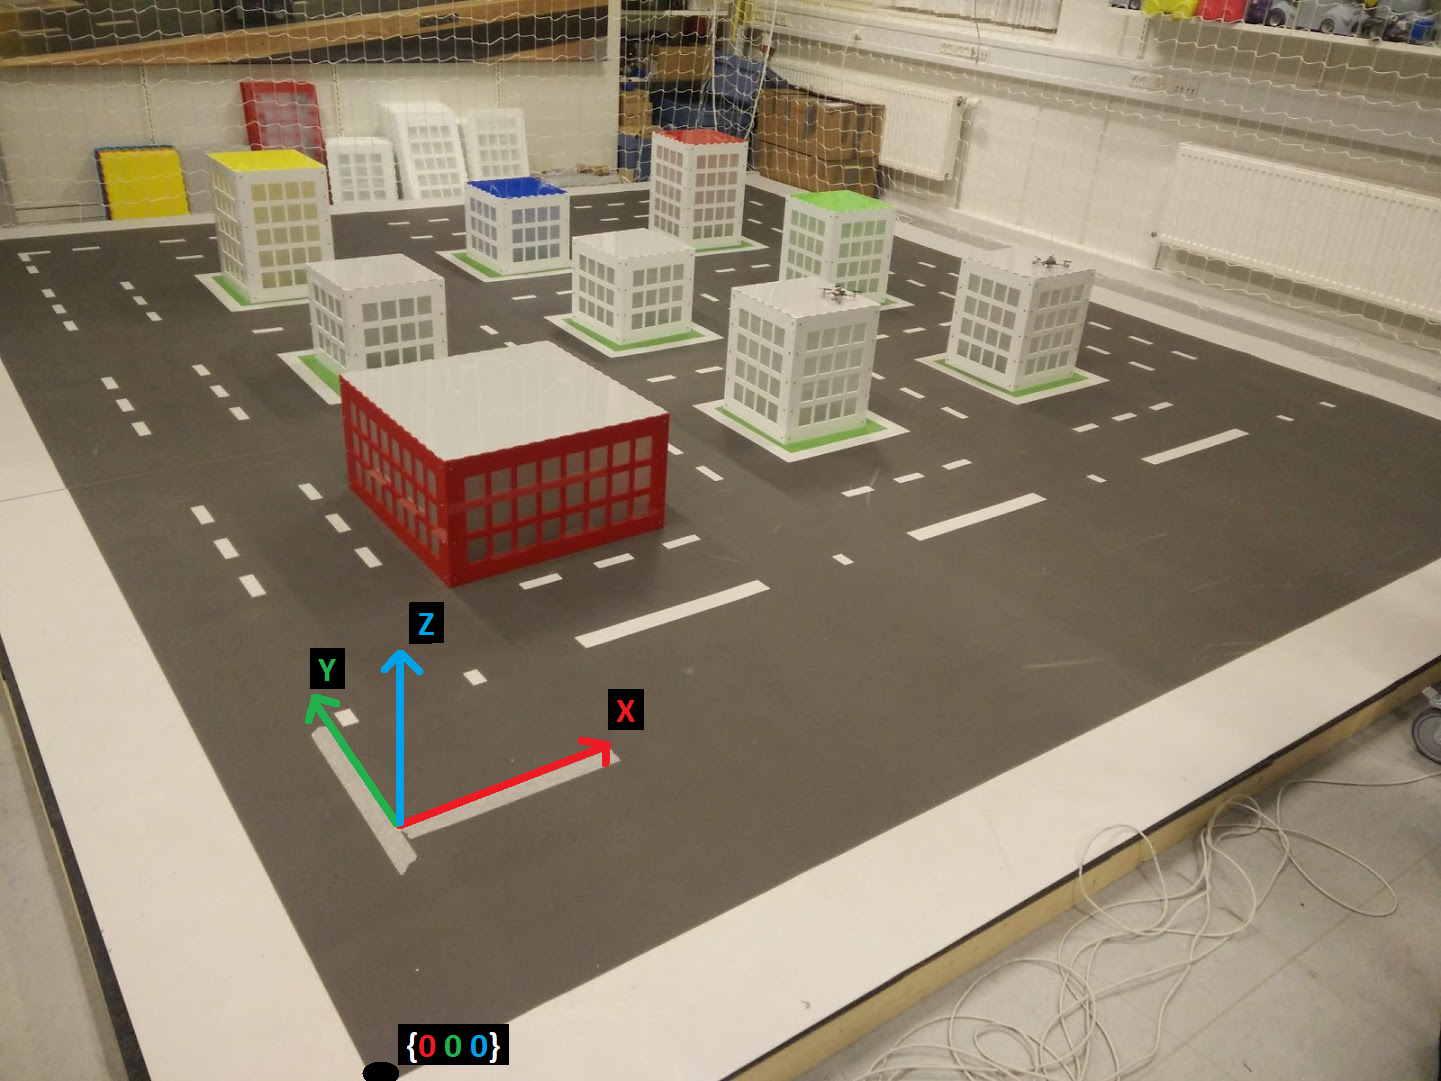
\includegraphics[width=\textwidth]{smartcity.png}
 \caption{Figure of the smart city setup. The direction of XYZ axes as well as the origin point can be observed.}
 \label{figure:smart_city_layout}
\end{figure}

The two crazyflie drones that execute the test flights are fitted with four reflective markers and Optitrack rigid bodies named \textit{crazyflie1} and \textit{crazyflie2} are created. Figure \ref{figure:optitrack_ui} shows the Optitrack Motive UI where the two drones from Figure \ref{figure:smart_city_layout} are being tracked.

\begin{figure}[H]
\centering
 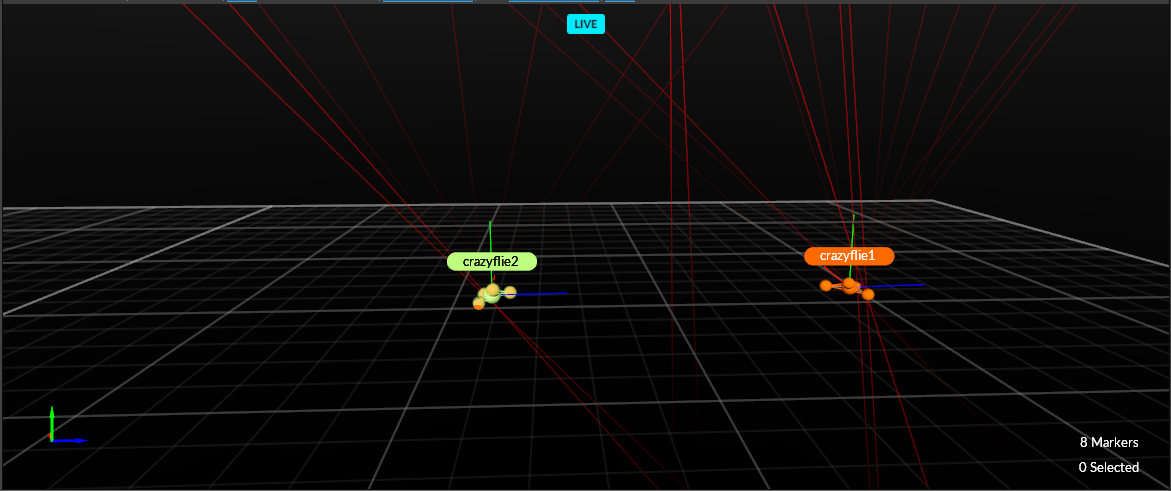
\includegraphics[width=\textwidth]{Figures/optitrack_ui.png}
 \caption{Optitrack Motive UI showing two tracked crazyflies.}
 \label{figure:optitrack_ui}
\end{figure}

\noindent where \textit{crazyflie1} is the drone on the bottom-right building and \textit{crazyflie2} is located on the bottom-center building.\\
\noindent At this point it is important to mention that the position axes in Optitrack are rotated differently than the ones in the SmartCity layout. A random drone position is taken in the SmartCity layout and the differences of representing that position are shown in Table \ref{table:smartcity-to-optitrack}.

\begin{table}[H]
\centering
\begin{tabular}{l|l|l|l|l|l|l|}
\cline{2-7}
 & \textbf{x} & \textbf{y} & \textbf{z} & \textbf{roll} & \textbf{pitch} & \textbf{yaw} \\ \cline{2-7} 
\multicolumn{1}{l|}{\textbf{Smart City}} & \cellcolor[HTML]{FE0000}{\color[HTML]{333333} 2.254} & \cellcolor[HTML]{67FD9A}1.711 & \cellcolor[HTML]{34CDF9}0.439 & 0 & 0 & \cellcolor[HTML]{F8FF00}84.392 \\ \cline{2-7} 
\multicolumn{1}{l|}{\textbf{Optitrack}} & \cellcolor[HTML]{67FD9A}1.711 & \cellcolor[HTML]{34CDF9}0.439 & \cellcolor[HTML]{FE0000}{\color[HTML]{333333} 2.254} & -24.999 & \cellcolor[HTML]{F8FF00}84.392 & -25.621 \\ \cline{2-7} 
\end{tabular}
\caption{Differences of representing a crazyflie position in SmartCity and Optitrack}
\label{table:smartcity-to-optitrack}
\end{table}

As Table \ref{table:smartcity-to-optitrack} shows there are key differences in how Optitrack reports the drone position. It can be noticed that the values are switched for $x$, $y$ and $z$-axis. The cause for the wrong $roll$ and $pitch$ values are because the current Optitrack setup reports them wrong. The values are switched since Optitrack reports the values in the $pitch, yaw, roll$ order while this project uses the $roll, pitch, yaw$ order.\\
The next section focuses on setting up the ROS environment to enable drone autonomous flight.
